% Options for packages loaded elsewhere
\PassOptionsToPackage{unicode}{hyperref}
\PassOptionsToPackage{hyphens}{url}
%
\documentclass[
]{article}
\usepackage{amsmath,amssymb}
\usepackage{lmodern}
\usepackage{iftex}
\ifPDFTeX
  \usepackage[T1]{fontenc}
  \usepackage[utf8]{inputenc}
  \usepackage{textcomp} % provide euro and other symbols
\else % if luatex or xetex
  \usepackage{unicode-math}
  \defaultfontfeatures{Scale=MatchLowercase}
  \defaultfontfeatures[\rmfamily]{Ligatures=TeX,Scale=1}
\fi
% Use upquote if available, for straight quotes in verbatim environments
\IfFileExists{upquote.sty}{\usepackage{upquote}}{}
\IfFileExists{microtype.sty}{% use microtype if available
  \usepackage[]{microtype}
  \UseMicrotypeSet[protrusion]{basicmath} % disable protrusion for tt fonts
}{}
\makeatletter
\@ifundefined{KOMAClassName}{% if non-KOMA class
  \IfFileExists{parskip.sty}{%
    \usepackage{parskip}
  }{% else
    \setlength{\parindent}{0pt}
    \setlength{\parskip}{6pt plus 2pt minus 1pt}}
}{% if KOMA class
  \KOMAoptions{parskip=half}}
\makeatother
\usepackage{xcolor}
\usepackage[margin=1in]{geometry}
\usepackage{color}
\usepackage{fancyvrb}
\newcommand{\VerbBar}{|}
\newcommand{\VERB}{\Verb[commandchars=\\\{\}]}
\DefineVerbatimEnvironment{Highlighting}{Verbatim}{commandchars=\\\{\}}
% Add ',fontsize=\small' for more characters per line
\usepackage{framed}
\definecolor{shadecolor}{RGB}{248,248,248}
\newenvironment{Shaded}{\begin{snugshade}}{\end{snugshade}}
\newcommand{\AlertTok}[1]{\textcolor[rgb]{0.94,0.16,0.16}{#1}}
\newcommand{\AnnotationTok}[1]{\textcolor[rgb]{0.56,0.35,0.01}{\textbf{\textit{#1}}}}
\newcommand{\AttributeTok}[1]{\textcolor[rgb]{0.77,0.63,0.00}{#1}}
\newcommand{\BaseNTok}[1]{\textcolor[rgb]{0.00,0.00,0.81}{#1}}
\newcommand{\BuiltInTok}[1]{#1}
\newcommand{\CharTok}[1]{\textcolor[rgb]{0.31,0.60,0.02}{#1}}
\newcommand{\CommentTok}[1]{\textcolor[rgb]{0.56,0.35,0.01}{\textit{#1}}}
\newcommand{\CommentVarTok}[1]{\textcolor[rgb]{0.56,0.35,0.01}{\textbf{\textit{#1}}}}
\newcommand{\ConstantTok}[1]{\textcolor[rgb]{0.00,0.00,0.00}{#1}}
\newcommand{\ControlFlowTok}[1]{\textcolor[rgb]{0.13,0.29,0.53}{\textbf{#1}}}
\newcommand{\DataTypeTok}[1]{\textcolor[rgb]{0.13,0.29,0.53}{#1}}
\newcommand{\DecValTok}[1]{\textcolor[rgb]{0.00,0.00,0.81}{#1}}
\newcommand{\DocumentationTok}[1]{\textcolor[rgb]{0.56,0.35,0.01}{\textbf{\textit{#1}}}}
\newcommand{\ErrorTok}[1]{\textcolor[rgb]{0.64,0.00,0.00}{\textbf{#1}}}
\newcommand{\ExtensionTok}[1]{#1}
\newcommand{\FloatTok}[1]{\textcolor[rgb]{0.00,0.00,0.81}{#1}}
\newcommand{\FunctionTok}[1]{\textcolor[rgb]{0.00,0.00,0.00}{#1}}
\newcommand{\ImportTok}[1]{#1}
\newcommand{\InformationTok}[1]{\textcolor[rgb]{0.56,0.35,0.01}{\textbf{\textit{#1}}}}
\newcommand{\KeywordTok}[1]{\textcolor[rgb]{0.13,0.29,0.53}{\textbf{#1}}}
\newcommand{\NormalTok}[1]{#1}
\newcommand{\OperatorTok}[1]{\textcolor[rgb]{0.81,0.36,0.00}{\textbf{#1}}}
\newcommand{\OtherTok}[1]{\textcolor[rgb]{0.56,0.35,0.01}{#1}}
\newcommand{\PreprocessorTok}[1]{\textcolor[rgb]{0.56,0.35,0.01}{\textit{#1}}}
\newcommand{\RegionMarkerTok}[1]{#1}
\newcommand{\SpecialCharTok}[1]{\textcolor[rgb]{0.00,0.00,0.00}{#1}}
\newcommand{\SpecialStringTok}[1]{\textcolor[rgb]{0.31,0.60,0.02}{#1}}
\newcommand{\StringTok}[1]{\textcolor[rgb]{0.31,0.60,0.02}{#1}}
\newcommand{\VariableTok}[1]{\textcolor[rgb]{0.00,0.00,0.00}{#1}}
\newcommand{\VerbatimStringTok}[1]{\textcolor[rgb]{0.31,0.60,0.02}{#1}}
\newcommand{\WarningTok}[1]{\textcolor[rgb]{0.56,0.35,0.01}{\textbf{\textit{#1}}}}
\usepackage{graphicx}
\makeatletter
\def\maxwidth{\ifdim\Gin@nat@width>\linewidth\linewidth\else\Gin@nat@width\fi}
\def\maxheight{\ifdim\Gin@nat@height>\textheight\textheight\else\Gin@nat@height\fi}
\makeatother
% Scale images if necessary, so that they will not overflow the page
% margins by default, and it is still possible to overwrite the defaults
% using explicit options in \includegraphics[width, height, ...]{}
\setkeys{Gin}{width=\maxwidth,height=\maxheight,keepaspectratio}
% Set default figure placement to htbp
\makeatletter
\def\fps@figure{htbp}
\makeatother
\setlength{\emergencystretch}{3em} % prevent overfull lines
\providecommand{\tightlist}{%
  \setlength{\itemsep}{0pt}\setlength{\parskip}{0pt}}
\setcounter{secnumdepth}{-\maxdimen} % remove section numbering
\ifLuaTeX
  \usepackage{selnolig}  % disable illegal ligatures
\fi
\IfFileExists{bookmark.sty}{\usepackage{bookmark}}{\usepackage{hyperref}}
\IfFileExists{xurl.sty}{\usepackage{xurl}}{} % add URL line breaks if available
\urlstyle{same} % disable monospaced font for URLs
\hypersetup{
  pdftitle={Compulsory exercise 1: Group 20},
  pdfauthor={Henrik Grenersen, Halvard Emil Sand-Larsen, Eirik Fagerbakke},
  hidelinks,
  pdfcreator={LaTeX via pandoc}}

\title{Compulsory exercise 1: Group 20}
\usepackage{etoolbox}
\makeatletter
\providecommand{\subtitle}[1]{% add subtitle to \maketitle
  \apptocmd{\@title}{\par {\large #1 \par}}{}{}
}
\makeatother
\subtitle{TMA4268 Statistical Learning V2023}
\author{Henrik Grenersen, Halvard Emil Sand-Larsen, Eirik Fagerbakke}
\date{22 februar, 2023}

\begin{document}
\maketitle

\begin{Shaded}
\begin{Highlighting}[]
\FunctionTok{library}\NormalTok{(knitr)}
\NormalTok{knitr}\SpecialCharTok{::}\NormalTok{opts\_chunk}\SpecialCharTok{$}\FunctionTok{set}\NormalTok{(}\AttributeTok{echo =} \ConstantTok{TRUE}\NormalTok{, }\AttributeTok{tidy=}\ConstantTok{TRUE}\NormalTok{,}\AttributeTok{message=}\ConstantTok{FALSE}\NormalTok{, }\AttributeTok{warning=}\ConstantTok{FALSE}\NormalTok{, }\AttributeTok{strip.white=}\ConstantTok{TRUE}\NormalTok{, }\AttributeTok{prompt=}\ConstantTok{FALSE}\NormalTok{,}
                      \AttributeTok{cache=}\ConstantTok{TRUE}\NormalTok{,  }\AttributeTok{size=}\StringTok{"scriptsize"}\NormalTok{,}\AttributeTok{fig.width=}\DecValTok{4}\NormalTok{, }\AttributeTok{fig.height=}\DecValTok{3}\NormalTok{,}\AttributeTok{fig.align =} \StringTok{"center"}\NormalTok{, }\AttributeTok{eval=}\ConstantTok{TRUE}\NormalTok{)}
\end{Highlighting}
\end{Shaded}

\begin{Shaded}
\begin{Highlighting}[]
\FunctionTok{install.packages}\NormalTok{(}\StringTok{"knitr"}\NormalTok{)  }\CommentTok{\# probably already installed}
\FunctionTok{install.packages}\NormalTok{(}\StringTok{"rmarkdown"}\NormalTok{)  }\CommentTok{\# probably already installed}
\FunctionTok{install.packages}\NormalTok{(}\StringTok{"ggplot2"}\NormalTok{)  }\CommentTok{\# plotting with ggplot2}
\FunctionTok{install.packages}\NormalTok{(}\StringTok{"dplyr"}\NormalTok{)  }\CommentTok{\# for data cleaning and preparation}
\FunctionTok{install.packages}\NormalTok{(}\StringTok{"tidyr"}\NormalTok{)  }\CommentTok{\# also data preparation}
\FunctionTok{install.packages}\NormalTok{(}\StringTok{"carData"}\NormalTok{)  }\CommentTok{\# dataset}
\FunctionTok{install.packages}\NormalTok{(}\StringTok{"class"}\NormalTok{)  }\CommentTok{\# for KNN}
\FunctionTok{install.packages}\NormalTok{(}\StringTok{"pROC"}\NormalTok{)  }\CommentTok{\# calculate roc}
\FunctionTok{install.packages}\NormalTok{(}\StringTok{"plotROC"}\NormalTok{)  }\CommentTok{\# plot roc}
\FunctionTok{install.packages}\NormalTok{(}\StringTok{"ggmosaic"}\NormalTok{)  }\CommentTok{\# mosaic plot}
\FunctionTok{install.packages}\NormalTok{(}\StringTok{"caret"}\NormalTok{)  }\CommentTok{\# functionality for confusion matrices}
\end{Highlighting}
\end{Shaded}

\hypertarget{problem-1}{%
\section{Problem 1}\label{problem-1}}

In this task we will consider \(Y = f(\bf{x}) + \epsilon\) where
\(\text{E}[\epsilon] = 0\) and \(\text{Var}[\epsilon] = \sigma^2\). For
this regression problem we will start with studying some properties of
some estimators for \(\beta\), namely \(\hat{\beta}\) and
\({\bf{\beta}}\).

\hypertarget{a}{%
\subsection{a)}\label{a}}

We will start with determining the expected value and variance of
\({\bf{\beta}}\). From our problem we have the following correlation. \[
E[\bf{Y}] = E[X \bf{\beta}+ \bf{\epsilon}] = X\bf{\beta} 
\] Using this, we get an expression for the expected value like this.

\[
\begin{aligned}
E[\tilde{\bf{\beta}}] &= E[(X^\top X+\lambda I)^{-1}X^\top \bf{Y}] \\
&=  (X^\top X+\lambda I)^{-1}X^\top E[\bf{Y}]\\
&=(X^\top X+\lambda I)^{-1}X^\top X \bf{\beta}\\
&= (X^\top X+\lambda I)^{-1} (X^\top X + \lambda I - \lambda I) \bf{\beta}\\
&= (X^\top X+\lambda I)^{-1} (X^\top X + \lambda I) \bf{\beta}- \lambda(X^\top X+\lambda I)^{-1} \beta\\
&= \bf{\beta}- \lambda(X^\top X+\lambda I)^{-1} \beta
\end{aligned}
\] We note that the estimator is biased, and now move on to the
variance.

\[
\begin{aligned}
\text{Var}[\tilde{\beta}]
&= \text{Var}[(X^\top X+\lambda I)^{-1}X^\top \bf{Y}]\\
&= (X^\top X+\lambda I)^{-1}X^\top \text{Var}[Y] ((X^\top X+\lambda I)^{-1}X^\top)^\top\\
&= \sigma^2 (X^\top X+\lambda I)^{-1}X^\top X (X^\top X+\lambda I)^{-\top}\\
&= \sigma^2 (X^\top X+\lambda I)^{-1} (X^\top X + \lambda I-\lambda I ) (X^\top X+\lambda I)^{-\top}\\
&= \sigma^2 \left((X^\top X+\lambda I)^{-1} (X^\top X+\lambda I) - \lambda(X^\top X+\lambda I)^{-1} \right)(X^\top X+\lambda I)^{-\top}\\
&= \sigma^2 (I -  \lambda(X^\top X+\lambda I)^{-1})(X^\top X+\lambda I)^{-\top}\\
\end{aligned}
\]

\hypertarget{b}{%
\subsection{b)}\label{b}}

We now want to consider the prediction \(\bf{x_0}^\top{\bf{\beta}}\),
denoted \({f}(\bf{x_0})\). And start with finding its expected value.

\[
E[\tilde{f}(\bf{x_0})] = E[\bf{x_0}^\top \tilde{\bf{\beta}}] = \bf{x_0}^\top (\bf{\beta}- \lambda(X^\top X+\lambda I)^{-1} \beta) 
\] We then find the variance as shown. \[
\text{Var}[\tilde{f}(\bf{x_0})] = \text{Var}[\bf{x_0}^\top \tilde{\bf{\beta}}] = \bf{x_0}^\top\text{Var}[ \tilde{\bf{\beta}}]\bf{x_0} = \sigma^2 \bf{x_0}^\top (I -  \lambda(X^\top X+\lambda I)^{-1})(X^\top X+\lambda I)^{-\top} \bf{x_0}
\]

\hypertarget{c}{%
\subsection{c)}\label{c}}

The bias of our method gives us an estimate of how our prediction
differs from the true mean.

The irreducible error stems from the random nature of the data set,
``noise'', and is normally represented by \(\epsilon\). As the name
suggests, it is irreducible.

The variance relates to the training of our method, and measures how
much our prediction would change for different training sets.

\hypertarget{d}{%
\subsection{d)}\label{d}}

We now want to find an expression for the MSE at \(x_0\), defined as
\$E{[}(y\_0-f(\bf{x_0}))^2] $.
$$
\begin{aligned}
E[(y_0 - \tilde{f}(\bf{x_0}))^2] 
&= \text{Var}[\epsilon] + \text{Var}[\tilde{f}(\bf{x}_0)] + (f(\bf{x}_0)-E[\tilde{f}(\bf{x}_0)])^2 \\
&= \sigma^2 \\
&+ \sigma^2 \bf{x_0}^\top (I -  \lambda(X^\top X+\lambda I)^{-1})(X^\top X+\lambda I)^{-\top} \bf{x_0} \\
&+ (\bf{x}_0^\top \beta -\bf{x_0}^\top (\bf{\beta}- \lambda(X^\top X+\lambda I)^{-1} \beta) )^2\\
&= \sigma^2 \left(1+ \bf{x_0}^\top (I -  \lambda(X^\top X+\lambda I)^{-1})(X^\top X+\lambda I)^{-\top} \bf{x_0} \right)\\
&+ (\bf{x_0}^\top \lambda(X^\top X+\lambda I)^{-1} \beta) )^2\\
\end{aligned}
$$

## e)
We now want to make a function to calculate the squared bias. To to this we firstly define the different paramaters we will need, and then fill in the handed out code with the proper expression.


```r
id <- "1X_8OKcoYbng1XvYFDirxjEWr7LtpNr1m"  # google file ID
values <- dget(sprintf("https://docs.google.com/uc?id=%s&export=download", id))

X <- values$X
dim(X)
```

\begin{verbatim}
## [1] 100  81
\end{verbatim}

\begin{Shaded}
\begin{Highlighting}[]
\NormalTok{x0 }\OtherTok{\textless{}{-}}\NormalTok{ values}\SpecialCharTok{$}\NormalTok{x0}
\FunctionTok{dim}\NormalTok{(x0)}
\end{Highlighting}
\end{Shaded}

\begin{verbatim}
## [1] 81  1
\end{verbatim}

\begin{Shaded}
\begin{Highlighting}[]
\NormalTok{beta }\OtherTok{\textless{}{-}}\NormalTok{ values}\SpecialCharTok{$}\NormalTok{beta}
\FunctionTok{dim}\NormalTok{(beta)}
\end{Highlighting}
\end{Shaded}

\begin{verbatim}
## [1] 81  1
\end{verbatim}

\begin{Shaded}
\begin{Highlighting}[]
\NormalTok{sigma }\OtherTok{\textless{}{-}}\NormalTok{ values}\SpecialCharTok{$}\NormalTok{sigma}
\NormalTok{sigma}
\end{Highlighting}
\end{Shaded}

\begin{verbatim}
## [1] 0.5
\end{verbatim}

\begin{Shaded}
\begin{Highlighting}[]
\FunctionTok{library}\NormalTok{(ggplot2)}
\NormalTok{bias }\OtherTok{\textless{}{-}} \ControlFlowTok{function}\NormalTok{(lambda, X, x0, beta) \{}
\NormalTok{    p }\OtherTok{\textless{}{-}} \FunctionTok{ncol}\NormalTok{(X)}
\NormalTok{    I }\OtherTok{=} \FunctionTok{diag}\NormalTok{(p)}
\NormalTok{    ridge\_inv }\OtherTok{\textless{}{-}} \FunctionTok{solve}\NormalTok{(}\FunctionTok{t}\NormalTok{(X) }\SpecialCharTok{\%*\%}\NormalTok{ X }\SpecialCharTok{+}\NormalTok{ lambda }\SpecialCharTok{*}\NormalTok{ I)}
\NormalTok{    value }\OtherTok{\textless{}{-}}\NormalTok{ (lambda }\SpecialCharTok{*} \FunctionTok{t}\NormalTok{(x0) }\SpecialCharTok{\%*\%}\NormalTok{ ridge\_inv }\SpecialCharTok{\%*\%}\NormalTok{ beta)}\SpecialCharTok{\^{}}\DecValTok{2}
    \FunctionTok{return}\NormalTok{(value)}
\NormalTok{\}}
\NormalTok{lambdas }\OtherTok{\textless{}{-}} \FunctionTok{seq}\NormalTok{(}\DecValTok{0}\NormalTok{, }\DecValTok{2}\NormalTok{, }\AttributeTok{length.out =} \DecValTok{500}\NormalTok{)}
\NormalTok{BIAS }\OtherTok{\textless{}{-}} \FunctionTok{rep}\NormalTok{(}\ConstantTok{NA}\NormalTok{, }\FunctionTok{length}\NormalTok{(lambdas))}
\ControlFlowTok{for}\NormalTok{ (i }\ControlFlowTok{in} \FunctionTok{seq\_along}\NormalTok{(lambdas)) BIAS[i] }\OtherTok{\textless{}{-}} \FunctionTok{bias}\NormalTok{(lambdas[i], X, x0, beta)}
\NormalTok{dfBias }\OtherTok{\textless{}{-}} \FunctionTok{data.frame}\NormalTok{(}\AttributeTok{lambdas =}\NormalTok{ lambdas, }\AttributeTok{bias =}\NormalTok{ BIAS)}
\FunctionTok{ggplot}\NormalTok{(dfBias, }\FunctionTok{aes}\NormalTok{(}\AttributeTok{x =}\NormalTok{ lambdas, }\AttributeTok{y =}\NormalTok{ bias)) }\SpecialCharTok{+} \FunctionTok{geom\_line}\NormalTok{(}\AttributeTok{color =} \StringTok{"hotpink"}\NormalTok{) }\SpecialCharTok{+} \FunctionTok{xlab}\NormalTok{(}\FunctionTok{expression}\NormalTok{(lambda)) }\SpecialCharTok{+}
    \FunctionTok{ylab}\NormalTok{(}\FunctionTok{expression}\NormalTok{(bias}\SpecialCharTok{\^{}}\DecValTok{2}\NormalTok{))}
\end{Highlighting}
\end{Shaded}

\begin{center}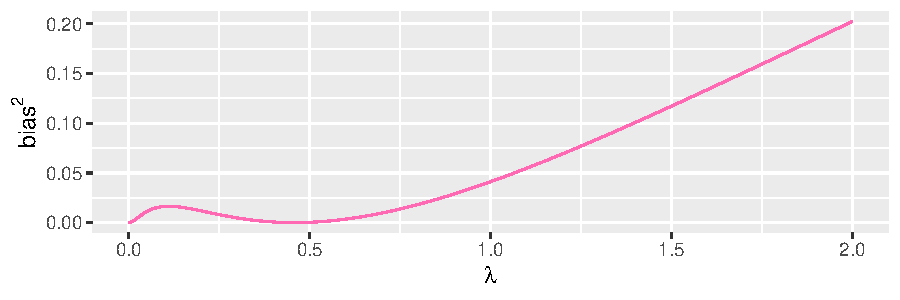
\includegraphics{Compulsory-1_files/figure-latex/unnamed-chunk-2-1} \end{center}

\hypertarget{f}{%
\subsection{f)}\label{f}}

Now we need a function for the variance, and as our parameters are
already defined above, we only need to fill in the handed out code.

\begin{Shaded}
\begin{Highlighting}[]
\NormalTok{variance }\OtherTok{\textless{}{-}} \ControlFlowTok{function}\NormalTok{(lambda, X, x0, sigma) \{}
\NormalTok{    p }\OtherTok{\textless{}{-}} \FunctionTok{ncol}\NormalTok{(X)}
\NormalTok{    I }\OtherTok{\textless{}{-}} \FunctionTok{diag}\NormalTok{(p)}
\NormalTok{    ridge\_inv }\OtherTok{\textless{}{-}} \FunctionTok{solve}\NormalTok{(}\FunctionTok{t}\NormalTok{(X) }\SpecialCharTok{\%*\%}\NormalTok{ X }\SpecialCharTok{+}\NormalTok{ lambda }\SpecialCharTok{*}\NormalTok{ I)}
\NormalTok{    value }\OtherTok{\textless{}{-}}\NormalTok{ sigma}\SpecialCharTok{\^{}}\DecValTok{2} \SpecialCharTok{*} \FunctionTok{t}\NormalTok{(x0) }\SpecialCharTok{\%*\%}\NormalTok{ (I }\SpecialCharTok{{-}}\NormalTok{ lambda }\SpecialCharTok{*}\NormalTok{ ridge\_inv) }\SpecialCharTok{\%*\%} \FunctionTok{t}\NormalTok{(ridge\_inv) }\SpecialCharTok{\%*\%}\NormalTok{ x0}
    \FunctionTok{return}\NormalTok{(value)}
\NormalTok{\}}
\NormalTok{lambdas }\OtherTok{\textless{}{-}} \FunctionTok{seq}\NormalTok{(}\DecValTok{0}\NormalTok{, }\DecValTok{2}\NormalTok{, }\AttributeTok{length.out =} \DecValTok{500}\NormalTok{)}
\NormalTok{VAR }\OtherTok{\textless{}{-}} \FunctionTok{rep}\NormalTok{(}\ConstantTok{NA}\NormalTok{, }\FunctionTok{length}\NormalTok{(lambdas))}
\ControlFlowTok{for}\NormalTok{ (i }\ControlFlowTok{in} \FunctionTok{seq\_along}\NormalTok{(lambdas)) VAR[i] }\OtherTok{\textless{}{-}} \FunctionTok{variance}\NormalTok{(lambdas[i], X, x0, sigma)}
\NormalTok{dfVar }\OtherTok{\textless{}{-}} \FunctionTok{data.frame}\NormalTok{(}\AttributeTok{lambdas =}\NormalTok{ lambdas, }\AttributeTok{var =}\NormalTok{ VAR)}
\FunctionTok{ggplot}\NormalTok{(dfVar, }\FunctionTok{aes}\NormalTok{(}\AttributeTok{x =}\NormalTok{ lambdas, }\AttributeTok{y =}\NormalTok{ var)) }\SpecialCharTok{+} \FunctionTok{geom\_line}\NormalTok{(}\AttributeTok{color =} \StringTok{"gold"}\NormalTok{) }\SpecialCharTok{+} \FunctionTok{xlab}\NormalTok{(}\FunctionTok{expression}\NormalTok{(lambda)) }\SpecialCharTok{+}
    \FunctionTok{ylab}\NormalTok{(}\StringTok{"variance"}\NormalTok{)}
\end{Highlighting}
\end{Shaded}

\begin{center}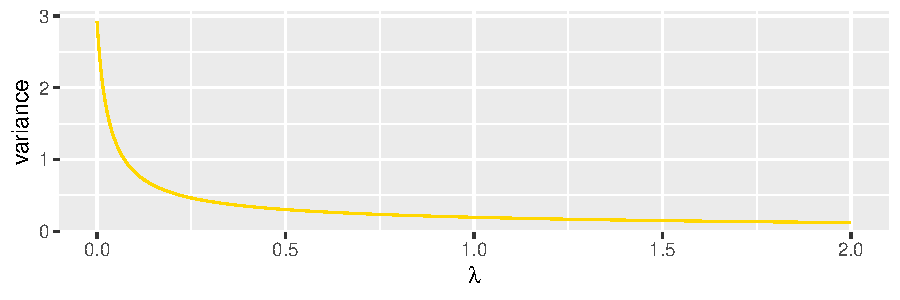
\includegraphics{Compulsory-1_files/figure-latex/unnamed-chunk-3-1} \end{center}

\hypertarget{g}{%
\subsection{g}\label{g}}

Combining the functions above we are able to calculate the MSE.

\begin{Shaded}
\begin{Highlighting}[]
\NormalTok{exp\_mse }\OtherTok{\textless{}{-}}\NormalTok{ sigma}\SpecialCharTok{\^{}}\DecValTok{2} \SpecialCharTok{+}\NormalTok{ VAR }\SpecialCharTok{+}\NormalTok{ BIAS}

\NormalTok{dfError }\OtherTok{=}\NormalTok{ dfVar}
\NormalTok{dfError}\SpecialCharTok{$}\NormalTok{MSE }\OtherTok{=}\NormalTok{ exp\_mse}
\NormalTok{dfError}\SpecialCharTok{$}\NormalTok{bias }\OtherTok{=}\NormalTok{ BIAS}

\FunctionTok{ggplot}\NormalTok{(dfError, }\FunctionTok{aes}\NormalTok{(}\AttributeTok{x =}\NormalTok{ lambdas)) }\SpecialCharTok{+} \FunctionTok{geom\_line}\NormalTok{(}\FunctionTok{aes}\NormalTok{(}\AttributeTok{y =}\NormalTok{ var), }\AttributeTok{color =} \StringTok{"gold"}\NormalTok{) }\SpecialCharTok{+} \FunctionTok{geom\_line}\NormalTok{(}\FunctionTok{aes}\NormalTok{(}\AttributeTok{y =}\NormalTok{ bias),}
    \AttributeTok{color =} \StringTok{"hotpink"}\NormalTok{) }\SpecialCharTok{+} \FunctionTok{geom\_line}\NormalTok{(}\FunctionTok{aes}\NormalTok{(}\AttributeTok{y =}\NormalTok{ MSE), }\AttributeTok{color =} \StringTok{"lightblue"}\NormalTok{) }\SpecialCharTok{+} \FunctionTok{xlab}\NormalTok{(}\FunctionTok{expression}\NormalTok{(lambda)) }\SpecialCharTok{+}
    \FunctionTok{ylab}\NormalTok{(}\StringTok{"errors"}\NormalTok{)}
\end{Highlighting}
\end{Shaded}

\begin{center}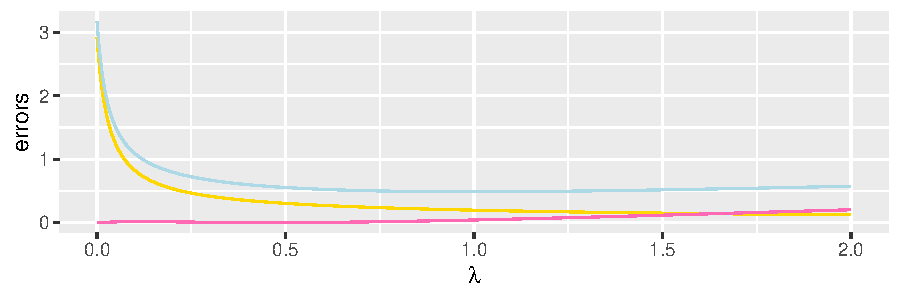
\includegraphics{Compulsory-1_files/figure-latex/unnamed-chunk-4-1} \end{center}

\begin{Shaded}
\begin{Highlighting}[]
\NormalTok{lambdas[}\FunctionTok{which.min}\NormalTok{(exp\_mse)]}
\end{Highlighting}
\end{Shaded}

\begin{verbatim}
## [1] 0.993988
\end{verbatim}

The lambda that corresponds to the smallest MSE is \(\lambda \approx\)
0.993988.

\hypertarget{problem-2}{%
\section{Problem 2}\label{problem-2}}

Here is a code chunk:

\begin{Shaded}
\begin{Highlighting}[]
\FunctionTok{library}\NormalTok{(carData)}
\CommentTok{\# ?Salaries}
\FunctionTok{data}\NormalTok{(Salaries)}
\NormalTok{GGally}\SpecialCharTok{::}\FunctionTok{ggpairs}\NormalTok{(Salaries)}
\end{Highlighting}
\end{Shaded}

\begin{figure}

{\centering 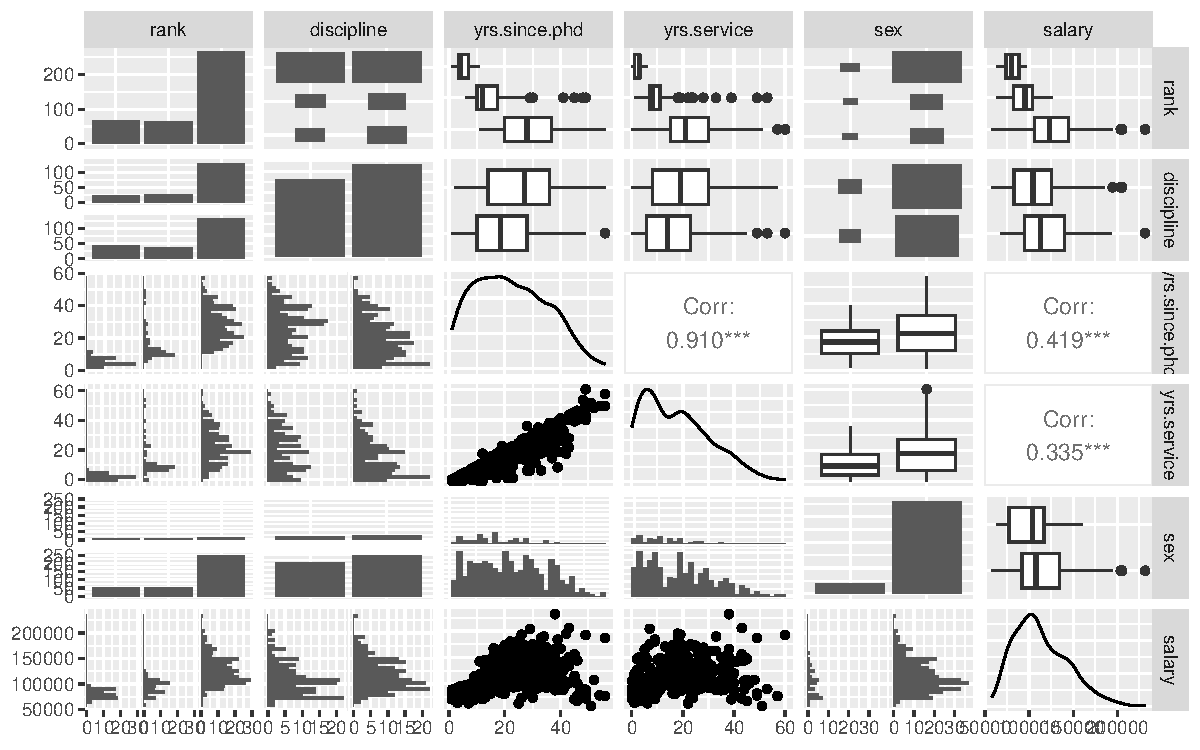
\includegraphics{Compulsory-1_files/figure-latex/desc-1} 

}

\caption{Pairs plot of the academic salary data set.}\label{fig:desc}
\end{figure}

\begin{Shaded}
\begin{Highlighting}[]
\CommentTok{\# Fit full model}
\NormalTok{model1 }\OtherTok{\textless{}{-}} \FunctionTok{lm}\NormalTok{(salary }\SpecialCharTok{\textasciitilde{}}\NormalTok{ ., }\AttributeTok{data =}\NormalTok{ Salaries)}
\FunctionTok{summary}\NormalTok{(model1)}
\end{Highlighting}
\end{Shaded}

\begin{verbatim}
## 
## Call:
## lm(formula = salary ~ ., data = Salaries)
## 
## Residuals:
##    Min     1Q Median     3Q    Max 
## -65248 -13211  -1775  10384  99592 
## 
## Coefficients:
##               Estimate Std. Error t value Pr(>|t|)    
## (Intercept)    65955.2     4588.6  14.374  < 2e-16 ***
## rankAssocProf  12907.6     4145.3   3.114  0.00198 ** 
## rankProf       45066.0     4237.5  10.635  < 2e-16 ***
## disciplineB    14417.6     2342.9   6.154 1.88e-09 ***
## yrs.since.phd    535.1      241.0   2.220  0.02698 *  
## yrs.service     -489.5      211.9  -2.310  0.02143 *  
## sexMale         4783.5     3858.7   1.240  0.21584    
## ---
## Signif. codes:  0 '***' 0.001 '**' 0.01 '*' 0.05 '.' 0.1 ' ' 1
## 
## Residual standard error: 22540 on 390 degrees of freedom
## Multiple R-squared:  0.4547, Adjusted R-squared:  0.4463 
## F-statistic:  54.2 on 6 and 390 DF,  p-value: < 2.2e-16
\end{verbatim}

\hypertarget{a-1}{%
\subsection{a)}\label{a-1}}

lm creates two dummy variables: ``rankAssocProf'' and ``rankProf''.
These are actually values compared to AsstProf as a baseline. This means
that if both dummy variables are zero, the individual is an assistant.
The coefficient for ``rankAssocProf'' thus represents an increase in
salary in our model for an individual that is an associate professor to
an assistant professor, and the case is the same for the ``rankProf''
coefficient, also compared to an assistant professor. If we had instead
chosen ``RankProf'' as our baseline, these coefficients would probably
be negative, as the other ranks have lower salaries compared to a full
professor.

To find the impact that rank has on salary as a whole, we perform an
F-test using anova. Here we test against the coefficients of both dummy
variables being set to zero.

\begin{Shaded}
\begin{Highlighting}[]
\NormalTok{Ftest.model1 }\OtherTok{=} \FunctionTok{anova}\NormalTok{(model1)}

\NormalTok{Ftest.model1[}\StringTok{"rank"}\NormalTok{, ]}\SpecialCharTok{$}\StringTok{\textasciigrave{}}\AttributeTok{Pr(\textgreater{}F)}\StringTok{\textasciigrave{}}
\end{Highlighting}
\end{Shaded}

\begin{verbatim}
## [1] 8.432273e-47
\end{verbatim}

Here we get a p-value of \ensuremath{8.4322731\times 10^{-47}}, which
means that it is highly likely that rank does have an effect on salary,
which is to be expected.

\hypertarget{b-1}{%
\subsection{b)}\label{b-1}}

From the descriptive analysis, we notice that there is a high
correlation between sex and rank, as well as between sex and
yrs.since.phd and yrs.service.

To invastigate this further, we plot sex against these three categories:

\begin{Shaded}
\begin{Highlighting}[]
\NormalTok{sex\_model }\OtherTok{\textless{}{-}} \FunctionTok{lm}\NormalTok{(salary }\SpecialCharTok{\textasciitilde{}}\NormalTok{ sex, }\AttributeTok{data =}\NormalTok{ Salaries)}
\FunctionTok{summary}\NormalTok{(sex\_model)}
\end{Highlighting}
\end{Shaded}

\begin{verbatim}
## 
## Call:
## lm(formula = salary ~ sex, data = Salaries)
## 
## Residuals:
##    Min     1Q Median     3Q    Max 
## -57290 -23502  -6828  19710 116455 
## 
## Coefficients:
##             Estimate Std. Error t value Pr(>|t|)    
## (Intercept)   101002       4809  21.001  < 2e-16 ***
## sexMale        14088       5065   2.782  0.00567 ** 
## ---
## Signif. codes:  0 '***' 0.001 '**' 0.01 '*' 0.05 '.' 0.1 ' ' 1
## 
## Residual standard error: 30030 on 395 degrees of freedom
## Multiple R-squared:  0.01921,    Adjusted R-squared:  0.01673 
## F-statistic: 7.738 on 1 and 395 DF,  p-value: 0.005667
\end{verbatim}

\begin{Shaded}
\begin{Highlighting}[]
\FunctionTok{par}\NormalTok{(}\AttributeTok{mfrow =} \FunctionTok{c}\NormalTok{(}\DecValTok{1}\NormalTok{, }\DecValTok{3}\NormalTok{))}
\FunctionTok{plot}\NormalTok{(sex }\SpecialCharTok{\textasciitilde{}}\NormalTok{ rank, }\AttributeTok{data =}\NormalTok{ Salaries)}
\FunctionTok{plot}\NormalTok{(sex }\SpecialCharTok{\textasciitilde{}}\NormalTok{ yrs.since.phd, }\AttributeTok{data =}\NormalTok{ Salaries)}
\FunctionTok{plot}\NormalTok{(sex }\SpecialCharTok{\textasciitilde{}}\NormalTok{ yrs.service, }\AttributeTok{data =}\NormalTok{ Salaries)}
\end{Highlighting}
\end{Shaded}

\begin{center}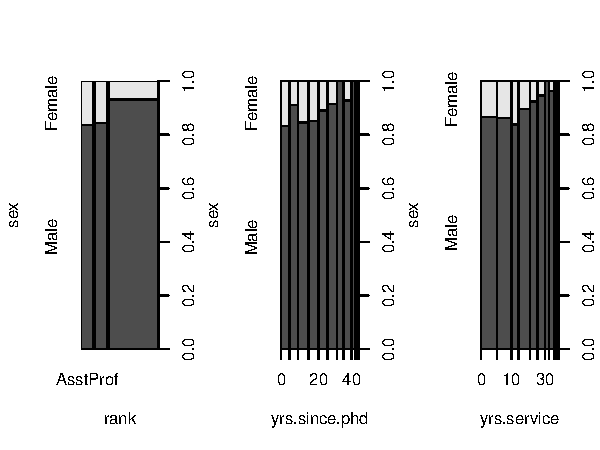
\includegraphics{Compulsory-1_files/figure-latex/unnamed-chunk-6-1} \end{center}

We see that the percentage of male individuals increases with rank,
yrs.since.phd and yrs.service. From the descriptive analysis and the
linear model, we have also seen that these three categories are
associated with a higher salary.

When we fit the linear model against all predictors, the effect of sex
might therefore be incorporated into other predictors. This gives rise
to the change in p-value that we see when fitting the linear model
against sex as our only predictor.

\hypertarget{c-1}{%
\subsection{c)}\label{c-1}}

\begin{Shaded}
\begin{Highlighting}[]
\FunctionTok{library}\NormalTok{(ggplot2)}
\FunctionTok{library}\NormalTok{(ggfortify)}
\FunctionTok{autoplot}\NormalTok{(model1, }\AttributeTok{smooth.colour =} \ConstantTok{NA}\NormalTok{)}
\end{Highlighting}
\end{Shaded}

\begin{center}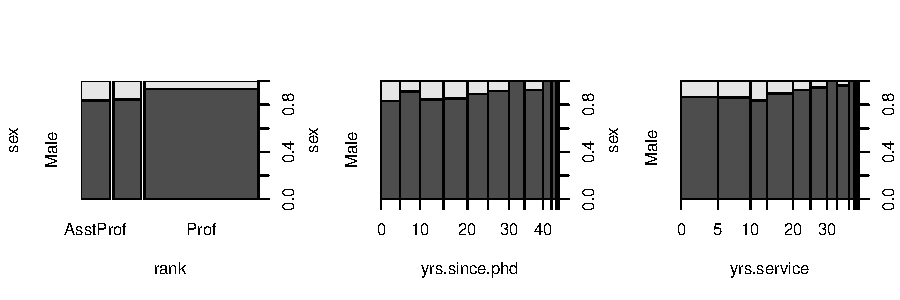
\includegraphics{Compulsory-1_files/figure-latex/unnamed-chunk-7-1} \end{center}

\hypertarget{i}{%
\subsubsection{i )}\label{i}}

From the residuals vs fitted-plot and the scale-location-plot, it looks
like the residuals are normally distributed. However, we see that the
variance increases with salary, which goes against our assumption of
homoscedasticity (all variances are equal).

The QQ-plot also does not seem entirely linear on the right side,
suggesting that the salary might not be normally distributed.

The residuals vs leverage-plot also suggests some outliers (250, 272,
331).

\hypertarget{ii}{%
\subsubsection{ii)}\label{ii}}

\begin{Shaded}
\begin{Highlighting}[]
\NormalTok{model2 }\OtherTok{\textless{}{-}} \FunctionTok{lm}\NormalTok{(}\FunctionTok{log}\NormalTok{(salary) }\SpecialCharTok{\textasciitilde{}}\NormalTok{ ., }\AttributeTok{data =}\NormalTok{ Salaries)}
\FunctionTok{summary}\NormalTok{(model2)}
\end{Highlighting}
\end{Shaded}

\begin{verbatim}
## 
## Call:
## lm(formula = log(salary) ~ ., data = Salaries)
## 
## Residuals:
##      Min       1Q   Median       3Q      Max 
## -0.66236 -0.10813 -0.00914  0.09804  0.60107 
## 
## Coefficients:
##                Estimate Std. Error t value Pr(>|t|)    
## (Intercept)   11.164144   0.036794 303.425  < 2e-16 ***
## rankAssocProf  0.153787   0.033239   4.627 5.06e-06 ***
## rankProf       0.449463   0.033979  13.228  < 2e-16 ***
## disciplineB    0.131869   0.018786   7.019 9.94e-12 ***
## yrs.since.phd  0.003289   0.001932   1.702   0.0896 .  
## yrs.service   -0.003918   0.001699  -2.305   0.0217 *  
## sexMale        0.045583   0.030941   1.473   0.1415    
## ---
## Signif. codes:  0 '***' 0.001 '**' 0.01 '*' 0.05 '.' 0.1 ' ' 1
## 
## Residual standard error: 0.1807 on 390 degrees of freedom
## Multiple R-squared:  0.5248, Adjusted R-squared:  0.5175 
## F-statistic: 71.79 on 6 and 390 DF,  p-value: < 2.2e-16
\end{verbatim}

\begin{Shaded}
\begin{Highlighting}[]
\FunctionTok{autoplot}\NormalTok{(model2, }\AttributeTok{smooth.colour =} \ConstantTok{NA}\NormalTok{)}
\end{Highlighting}
\end{Shaded}

\begin{center}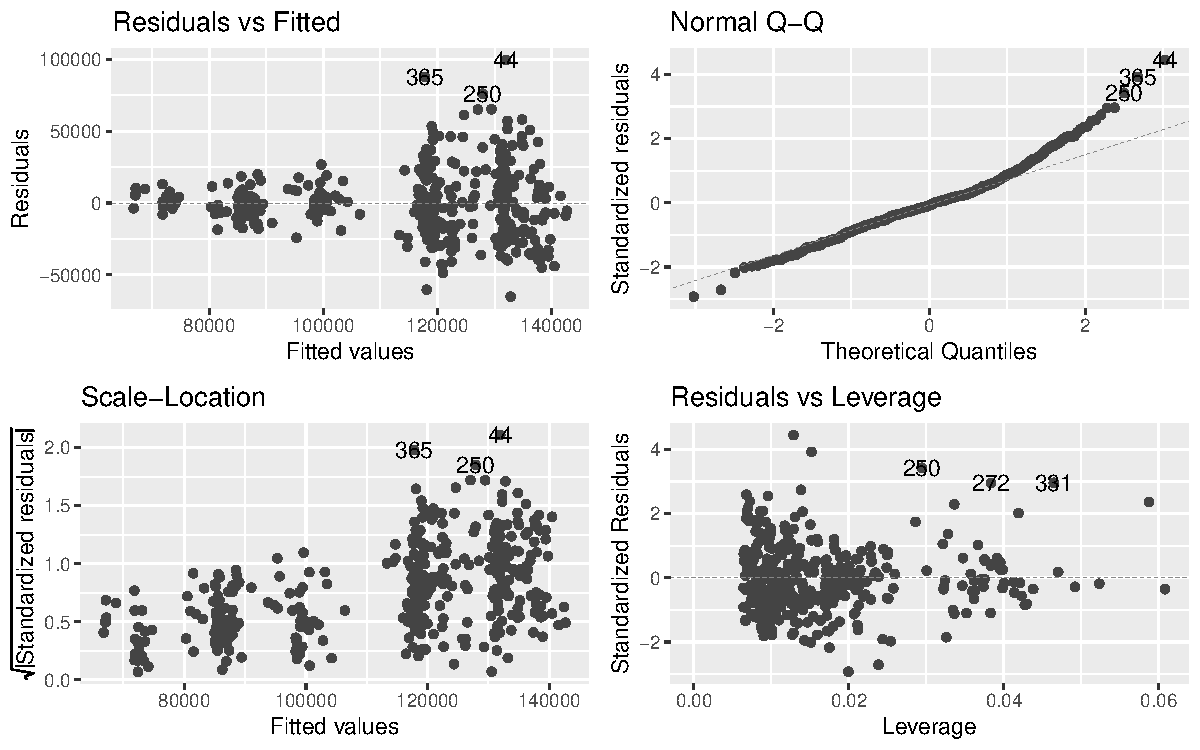
\includegraphics{Compulsory-1_files/figure-latex/unnamed-chunk-8-1} \end{center}

In these plots we see that have a straighter line in our QQ-plot,
implying that our data seems more normally distributed than previously.
Thus, the model assumptions have improved slightly when taking the log
of our response and including all predictors.

\hypertarget{d-1}{%
\subsection{d)}\label{d-1}}

\hypertarget{i-1}{%
\subsubsection{i)}\label{i-1}}

\begin{Shaded}
\begin{Highlighting}[]
\NormalTok{model3 }\OtherTok{\textless{}{-}} \FunctionTok{lm}\NormalTok{(}\FunctionTok{log}\NormalTok{(salary) }\SpecialCharTok{\textasciitilde{}}\NormalTok{ . }\SpecialCharTok{+}\NormalTok{ sex}\SpecialCharTok{:}\NormalTok{yrs.since.phd, }\AttributeTok{data =}\NormalTok{ Salaries)}
\FunctionTok{summary}\NormalTok{(model3)}
\end{Highlighting}
\end{Shaded}

\begin{verbatim}
## 
## Call:
## lm(formula = log(salary) ~ . + sex:yrs.since.phd, data = Salaries)
## 
## Residuals:
##      Min       1Q   Median       3Q      Max 
## -0.66187 -0.10831 -0.00951  0.09846  0.60143 
## 
## Coefficients:
##                         Estimate Std. Error t value Pr(>|t|)    
## (Intercept)           11.1537511  0.0591759 188.485  < 2e-16 ***
## rankAssocProf          0.1528200  0.0335575   4.554 7.05e-06 ***
## rankProf               0.4482679  0.0344343  13.018  < 2e-16 ***
## disciplineB            0.1317818  0.0188133   7.005 1.09e-11 ***
## yrs.since.phd          0.0039500  0.0035253   1.120   0.2632    
## yrs.service           -0.0038902  0.0017059  -2.280   0.0231 *  
## sexMale                0.0574914  0.0614436   0.936   0.3500    
## yrs.since.phd:sexMale -0.0007049  0.0031407  -0.224   0.8225    
## ---
## Signif. codes:  0 '***' 0.001 '**' 0.01 '*' 0.05 '.' 0.1 ' ' 1
## 
## Residual standard error: 0.1809 on 389 degrees of freedom
## Multiple R-squared:  0.5249, Adjusted R-squared:  0.5163 
## F-statistic: 61.39 on 7 and 389 DF,  p-value: < 2.2e-16
\end{verbatim}

\hypertarget{ii-1}{%
\subsubsection{ii)}\label{ii-1}}

We observe a quite large p-value for the interaction term.

\begin{Shaded}
\begin{Highlighting}[]
\FunctionTok{print}\NormalTok{(}\FunctionTok{anova}\NormalTok{(model2, model3))}
\end{Highlighting}
\end{Shaded}

\begin{verbatim}
## Analysis of Variance Table
## 
## Model 1: log(salary) ~ rank + discipline + yrs.since.phd + yrs.service + 
##     sex
## Model 2: log(salary) ~ rank + discipline + yrs.since.phd + yrs.service + 
##     sex + sex:yrs.since.phd
##   Res.Df    RSS Df Sum of Sq      F Pr(>F)
## 1    390 12.738                           
## 2    389 12.736  1 0.0016491 0.0504 0.8225
\end{verbatim}

Comparing our model with all predictors with the new one where we have
added the interaction term, we again observe a quite large p-value,
which indicates that the difference in the models' performances is
non-significant, and we should stick to our simpler, original model, and
reject Bert-Ernie's hypothesis.

\hypertarget{e}{%
\subsection{e)}\label{e}}

\begin{Shaded}
\begin{Highlighting}[]
\FunctionTok{set.seed}\NormalTok{(}\DecValTok{4268}\NormalTok{)}

\NormalTok{B }\OtherTok{\textless{}{-}} \DecValTok{1000}

\NormalTok{Rs }\OtherTok{\textless{}{-}} \FunctionTok{rep}\NormalTok{(}\ConstantTok{NA}\NormalTok{, B)}

\ControlFlowTok{for}\NormalTok{ (b }\ControlFlowTok{in} \DecValTok{1}\SpecialCharTok{:}\NormalTok{B) \{}
\NormalTok{    boot.sample }\OtherTok{\textless{}{-}}\NormalTok{ Salaries[}\FunctionTok{sample}\NormalTok{(}\DecValTok{1}\SpecialCharTok{:}\FunctionTok{dim}\NormalTok{(Salaries)[}\DecValTok{1}\NormalTok{], }\AttributeTok{replace =} \ConstantTok{TRUE}\NormalTok{), ]}
\NormalTok{    boot.fit }\OtherTok{\textless{}{-}} \FunctionTok{lm}\NormalTok{(}\FunctionTok{log}\NormalTok{(salary) }\SpecialCharTok{\textasciitilde{}}\NormalTok{ ., }\AttributeTok{data =}\NormalTok{ boot.sample)}
\NormalTok{    boot.sum }\OtherTok{\textless{}{-}} \FunctionTok{summary}\NormalTok{(boot.fit)}
\NormalTok{    Rs[b] }\OtherTok{\textless{}{-}}\NormalTok{ boot.sum}\SpecialCharTok{$}\NormalTok{r.squared}
\NormalTok{\}}
\NormalTok{standard\_error }\OtherTok{\textless{}{-}} \FunctionTok{sd}\NormalTok{(Rs)}
\NormalTok{Se }\OtherTok{\textless{}{-}}\NormalTok{ standard\_error}

\NormalTok{quant }\OtherTok{\textless{}{-}} \FunctionTok{quantile}\NormalTok{(Rs, }\FunctionTok{c}\NormalTok{(}\FloatTok{0.025}\NormalTok{, }\FloatTok{0.975}\NormalTok{))}

\NormalTok{Rs.df }\OtherTok{\textless{}{-}} \FunctionTok{data.frame}\NormalTok{(}\AttributeTok{Rs =}\NormalTok{ Rs, }\AttributeTok{norm\_den =} \FunctionTok{dnorm}\NormalTok{(Rs, }\FunctionTok{mean}\NormalTok{(Rs), }\FunctionTok{sd}\NormalTok{(Rs)))}

\FunctionTok{ggplot}\NormalTok{(Rs.df) }\SpecialCharTok{+} \FunctionTok{geom\_histogram}\NormalTok{(}\FunctionTok{aes}\NormalTok{(}\AttributeTok{x =}\NormalTok{ Rs, }\AttributeTok{y =}\NormalTok{ ..density..), }\AttributeTok{fill =} \StringTok{"grey80"}\NormalTok{, }\AttributeTok{color =} \StringTok{"black"}\NormalTok{) }\SpecialCharTok{+}
    \FunctionTok{ggtitle}\NormalTok{(}\FunctionTok{expression}\NormalTok{(R}\SpecialCharTok{\^{}}\DecValTok{2}\NormalTok{)) }\SpecialCharTok{+} \FunctionTok{geom\_line}\NormalTok{(}\FunctionTok{aes}\NormalTok{(}\AttributeTok{x =}\NormalTok{ Rs, }\AttributeTok{y =}\NormalTok{ norm\_den), }\AttributeTok{color =} \StringTok{"red"}\NormalTok{) }\SpecialCharTok{+}
    \FunctionTok{theme\_minimal}\NormalTok{()}
\end{Highlighting}
\end{Shaded}

\begin{center}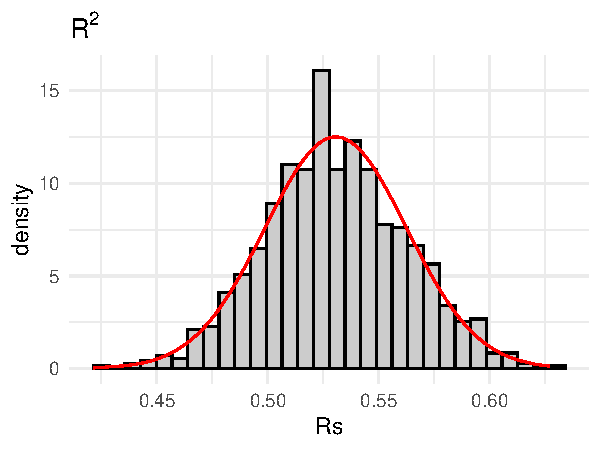
\includegraphics{Compulsory-1_files/figure-latex/unnamed-chunk-11-1} \end{center}

In the above chunks we found the following standard error: 0.031911 and
the 95\% quantile interval: {[}0.4691091, 0.5945034{]}. From our
histogram of R squared we also see that the values are approximately
normally distributed and that our values are rather small, which
indicates that our model is not an especially good fit for our data.

\hypertarget{f-1}{%
\subsection{f)}\label{f-1}}

\begin{Shaded}
\begin{Highlighting}[]
\CommentTok{\#Code provided in exercise}
\CommentTok{\# Make a data frame containing two new observations, corresponding to}
\CommentTok{\# Bert{-}Ernie\textquotesingle{}s two possible futures}
\NormalTok{bert\_ernie }\OtherTok{\textless{}{-}} \FunctionTok{data.frame}\NormalTok{(}\AttributeTok{rank =} \FunctionTok{c}\NormalTok{(}\StringTok{"Prof"}\NormalTok{, }\StringTok{"Prof"}\NormalTok{),}
\AttributeTok{discipline =} \FunctionTok{c}\NormalTok{(}\StringTok{"A"}\NormalTok{, }\StringTok{"B"}\NormalTok{), }\CommentTok{\# Theoretical, applied}
\AttributeTok{yrs.since.phd =} \FunctionTok{c}\NormalTok{(}\DecValTok{20}\NormalTok{, }\DecValTok{20}\NormalTok{),}
\AttributeTok{yrs.service =} \FunctionTok{c}\NormalTok{(}\DecValTok{20}\NormalTok{, }\DecValTok{20}\NormalTok{),}
\AttributeTok{sex =} \FunctionTok{c}\NormalTok{(}\StringTok{"Male"}\NormalTok{, }\StringTok{"Male"}\NormalTok{))}
\CommentTok{\# Use the full model to predict his salary}
\NormalTok{preds }\OtherTok{\textless{}{-}} \FunctionTok{predict}\NormalTok{(}\AttributeTok{object =}\NormalTok{ model1,}
\AttributeTok{newdata =}\NormalTok{ bert\_ernie,}
\AttributeTok{interval =} \StringTok{"prediction"}\NormalTok{,}
\AttributeTok{level =} \FloatTok{0.9}\NormalTok{) }
\CommentTok{\# Check predictions}
\NormalTok{preds}
\end{Highlighting}
\end{Shaded}

\begin{verbatim}
##        fit      lwr      upr
## 1 116715.6 79318.04 154113.1
## 2 131133.2 93792.87 168473.5
\end{verbatim}

\begin{Shaded}
\begin{Highlighting}[]
\FunctionTok{summary}\NormalTok{(model1)}
\end{Highlighting}
\end{Shaded}

\begin{verbatim}
## 
## Call:
## lm(formula = salary ~ ., data = Salaries)
## 
## Residuals:
##    Min     1Q Median     3Q    Max 
## -65248 -13211  -1775  10384  99592 
## 
## Coefficients:
##               Estimate Std. Error t value Pr(>|t|)    
## (Intercept)    65955.2     4588.6  14.374  < 2e-16 ***
## rankAssocProf  12907.6     4145.3   3.114  0.00198 ** 
## rankProf       45066.0     4237.5  10.635  < 2e-16 ***
## disciplineB    14417.6     2342.9   6.154 1.88e-09 ***
## yrs.since.phd    535.1      241.0   2.220  0.02698 *  
## yrs.service     -489.5      211.9  -2.310  0.02143 *  
## sexMale         4783.5     3858.7   1.240  0.21584    
## ---
## Signif. codes:  0 '***' 0.001 '**' 0.01 '*' 0.05 '.' 0.1 ' ' 1
## 
## Residual standard error: 22540 on 390 degrees of freedom
## Multiple R-squared:  0.4547, Adjusted R-squared:  0.4463 
## F-statistic:  54.2 on 6 and 390 DF,  p-value: < 2.2e-16
\end{verbatim}

\hypertarget{i-2}{%
\subsubsection{i)}\label{i-2}}

The only things we changed in the above code snippet was that we changed
the arguments interval to ``prediction'' and level to 0.9. Because the
lower value is \ensuremath{7.9318035\times 10^{4}}, he should be able to
follow his dream.

\hypertarget{ii-2}{%
\subsubsection{ii)}\label{ii-2}}

Our analytic expression for the correct lower limit is: \[
\text{limit}_\text{lower} = \text{E[Bert-Ernie's salary]} - t_{n-p, 0.9} \hat{\sigma}\sqrt{1+x_0^\top(X^\top X)^{-1}x_0}
\] \[
\quad n=\text{number of observations} \quad \text{p=number of predictors}
\] Where in our case, \$n-p=\$391. As an estimator of the variance, we
have used \[
H =X(X^\top X)^{-1}X^\top
\] \[
\hat{\epsilon} = (I-H)Y
\] \[
\hat{\sigma}^2 = \frac{1}{n-p}\hat{\epsilon}^\top\hat{\epsilon}
\] We have calculated this value in the chunk below:

\begin{Shaded}
\begin{Highlighting}[]
\NormalTok{A }\OtherTok{\textless{}{-}} \FunctionTok{data.matrix}\NormalTok{(Salaries[, }\SpecialCharTok{!}\FunctionTok{names}\NormalTok{(Salaries) }\SpecialCharTok{\%in\%} \FunctionTok{c}\NormalTok{(}\StringTok{"salary"}\NormalTok{)])}
\NormalTok{X }\OtherTok{\textless{}{-}} \FunctionTok{model.matrix}\NormalTok{(model1)}

\NormalTok{n }\OtherTok{\textless{}{-}} \FunctionTok{dim}\NormalTok{(X)[}\DecValTok{1}\NormalTok{]}
\NormalTok{p }\OtherTok{\textless{}{-}} \FunctionTok{dim}\NormalTok{(X)[}\DecValTok{2}\NormalTok{]}


\NormalTok{Y }\OtherTok{\textless{}{-}} \FunctionTok{data.matrix}\NormalTok{(Salaries[, }\StringTok{"salary"}\NormalTok{])}

\NormalTok{x0 }\OtherTok{\textless{}{-}} \FunctionTok{data.matrix}\NormalTok{(bert\_ernie)[}\DecValTok{1}\NormalTok{, ]}
\NormalTok{x0 }\OtherTok{\textless{}{-}} \FunctionTok{c}\NormalTok{(}\DecValTok{1}\NormalTok{, }\DecValTok{0}\NormalTok{, x0)}

\NormalTok{mu0 }\OtherTok{\textless{}{-}} \FunctionTok{predict}\NormalTok{(}\AttributeTok{object =}\NormalTok{ model1, }\AttributeTok{newdata =}\NormalTok{ bert\_ernie[}\DecValTok{1}\NormalTok{, ])  }\CommentTok{\#expected value}
\NormalTok{t }\OtherTok{\textless{}{-}} \FunctionTok{qt}\NormalTok{(}\DecValTok{1} \SpecialCharTok{{-}} \FloatTok{0.1}\SpecialCharTok{/}\DecValTok{2}\NormalTok{, n }\SpecialCharTok{{-}}\NormalTok{ p)  }\CommentTok{\#t{-}value for one{-}sided 95\% pred int}

\NormalTok{H }\OtherTok{\textless{}{-}}\NormalTok{ X }\SpecialCharTok{\%*\%} \FunctionTok{solve}\NormalTok{(}\FunctionTok{t}\NormalTok{(X) }\SpecialCharTok{\%*\%}\NormalTok{ X) }\SpecialCharTok{\%*\%} \FunctionTok{t}\NormalTok{(X)}
\NormalTok{epsilon\_hat }\OtherTok{\textless{}{-}}\NormalTok{ (}\FunctionTok{diag}\NormalTok{(n) }\SpecialCharTok{{-}}\NormalTok{ H) }\SpecialCharTok{\%*\%}\NormalTok{ Y}

\NormalTok{sigma\_hat }\OtherTok{\textless{}{-}} \FunctionTok{sqrt}\NormalTok{(}\DecValTok{1}\SpecialCharTok{/}\NormalTok{(n }\SpecialCharTok{{-}}\NormalTok{ p) }\SpecialCharTok{*} \FunctionTok{t}\NormalTok{(epsilon\_hat) }\SpecialCharTok{\%*\%}\NormalTok{ epsilon\_hat)  }\CommentTok{\#disse er ikke like!}
\NormalTok{sigma\_hat}
\end{Highlighting}
\end{Shaded}

\begin{verbatim}
##          [,1]
## [1,] 22538.65
\end{verbatim}

\begin{Shaded}
\begin{Highlighting}[]
\CommentTok{\# sigma\_hat \textless{}{-} summary(model1)$sigma sigma\_hat}
\NormalTok{pred\_lwr }\OtherTok{\textless{}{-}}\NormalTok{ mu0 }\SpecialCharTok{{-}}\NormalTok{ t }\SpecialCharTok{*}\NormalTok{ sigma\_hat }\SpecialCharTok{*} \FunctionTok{sqrt}\NormalTok{(}\DecValTok{1} \SpecialCharTok{+} \FunctionTok{t}\NormalTok{(x0) }\SpecialCharTok{\%*\%} \FunctionTok{solve}\NormalTok{(}\FunctionTok{t}\NormalTok{(X) }\SpecialCharTok{\%*\%}\NormalTok{ X) }\SpecialCharTok{\%*\%}\NormalTok{ x0)}

\NormalTok{pred\_lwr}
\end{Highlighting}
\end{Shaded}

\begin{verbatim}
##          [,1]
## [1,] 79375.24
\end{verbatim}

\begin{Shaded}
\begin{Highlighting}[]
\CommentTok{\# limit\_theoretical \textless{}{-} predict(object = model1, newdata = bert\_ernie) {-}}
\CommentTok{\# rep(qt(0.9, n{-}p),1)*sqrt(sigma\_hat +}
\CommentTok{\# sigma\_hat*(data.matrix(bert\_ernie))\%*\%solve(t(X)\%*\%X)\%*\%t(data.matrix(bert\_ernie)))}
\CommentTok{\# limit\_theoretical}
\NormalTok{model1}\SpecialCharTok{$}\NormalTok{df.residual}
\end{Highlighting}
\end{Shaded}

\begin{verbatim}
## [1] 390
\end{verbatim}

\hypertarget{problem-3}{%
\section{Problem 3}\label{problem-3}}

In this task we will help the Bigfoot Field Researchers Organization
(BFRO) with automating their process for classifying reported sightings
of Bigfoots. In the chunk below we use code that was provided to us in
order to tidy up our data and make it easier to work with.

\begin{Shaded}
\begin{Highlighting}[]
\CommentTok{\# The code in this chunk was provided in the exercise}

\NormalTok{bigfoot\_original }\OtherTok{\textless{}{-}}\NormalTok{ readr}\SpecialCharTok{::}\FunctionTok{read\_csv}\NormalTok{(}\StringTok{"https://raw.githubusercontent.com/rfordatascience/tidytuesday/master/data/2022/2022{-}09{-}13/bigfoot.csv"}\NormalTok{)}
\FunctionTok{summary}\NormalTok{(bigfoot\_original)}
\end{Highlighting}
\end{Shaded}

\begin{verbatim}
##    observed         location_details      county             state          
##  Length:5021        Length:5021        Length:5021        Length:5021       
##  Class :character   Class :character   Class :character   Class :character  
##  Mode  :character   Mode  :character   Mode  :character   Mode  :character  
##                                                                             
##                                                                             
##                                                                             
##                                                                             
##     season             title              latitude       longitude      
##  Length:5021        Length:5021        Min.   :25.14   Min.   :-167.13  
##  Class :character   Class :character   1st Qu.:35.35   1st Qu.:-117.06  
##  Mode  :character   Mode  :character   Median :39.30   Median : -91.77  
##                                        Mean   :39.36   Mean   : -97.42  
##                                        3rd Qu.:43.93   3rd Qu.: -83.07  
##                                        Max.   :64.89   Max.   : -68.23  
##                                        NA's   :976     NA's   :976      
##       date                number      classification       geohash         
##  Min.   :1869-11-10   Min.   :   60   Length:5021        Length:5021       
##  1st Qu.:1990-09-15   1st Qu.: 4595   Class :character   Class :character  
##  Median :2003-11-16   Median :15473   Mode  :character   Mode  :character  
##  Mean   :1999-06-22   Mean   :21520                                        
##  3rd Qu.:2009-08-16   3rd Qu.:33979                                        
##  Max.   :2021-11-27   Max.   :71997                                        
##  NA's   :976                                                               
##  temperature_high temperature_mid  temperature_low    dew_point     
##  Min.   : -0.62   Min.   :-8.455   Min.   :-22.78   Min.   :-11.21  
##  1st Qu.: 55.14   1st Qu.:46.767   1st Qu.: 37.50   1st Qu.: 34.77  
##  Median : 69.97   Median :59.360   Median : 49.40   Median : 46.69  
##  Mean   : 67.12   Mean   :57.843   Mean   : 48.64   Mean   : 46.23  
##  3rd Qu.: 81.09   3rd Qu.:70.380   3rd Qu.: 60.66   3rd Qu.: 59.00  
##  Max.   :106.51   Max.   :94.030   Max.   : 84.34   Max.   : 77.40  
##  NA's   :1683     NA's   :1835     NA's   :1832     NA's   :1648    
##     humidity       cloud_cover      moon_phase    precip_intensity
##  Min.   :0.0800   Min.   :0.000   Min.   :0.000   Min.   :0.0000  
##  1st Qu.:0.6200   1st Qu.:0.120   1st Qu.:0.250   1st Qu.:0.0000  
##  Median :0.7300   Median :0.400   Median :0.490   Median :0.0000  
##  Mean   :0.7057   Mean   :0.439   Mean   :0.498   Mean   :0.0057  
##  3rd Qu.:0.8200   3rd Qu.:0.730   3rd Qu.:0.750   3rd Qu.:0.0015  
##  Max.   :1.0000   Max.   :1.000   Max.   :1.000   Max.   :2.0690  
##  NA's   :1648     NA's   :1937    NA's   :1625    NA's   :2309    
##  precip_probability precip_type           pressure        summary         
##  Min.   :0.0000     Length:5021        Min.   : 980.3   Length:5021       
##  1st Qu.:0.0000     Class :character   1st Qu.:1013.4   Class :character  
##  Median :0.0000     Mode  :character   Median :1017.0   Mode  :character  
##  Mean   :0.2958                        Mean   :1017.1                     
##  3rd Qu.:0.7300                        3rd Qu.:1020.6                     
##  Max.   :1.0000                        Max.   :1042.4                     
##  NA's   :2311                          NA's   :2402                       
##     uv_index        visibility      wind_bearing     wind_speed    
##  Min.   : 0.000   Min.   : 0.740   Min.   :  0.0   Min.   : 0.000  
##  1st Qu.: 3.000   1st Qu.: 7.660   1st Qu.:128.0   1st Qu.: 1.340  
##  Median : 5.000   Median : 9.451   Median :203.0   Median : 2.930  
##  Mean   : 5.161   Mean   : 8.492   Mean   :196.6   Mean   : 3.866  
##  3rd Qu.: 8.000   3rd Qu.:10.000   3rd Qu.:273.0   3rd Qu.: 5.560  
##  Max.   :13.000   Max.   :10.000   Max.   :359.0   Max.   :23.940  
##  NA's   :1629     NA's   :1972     NA's   :1634    NA's   :1632
\end{verbatim}

\begin{Shaded}
\begin{Highlighting}[]
\CommentTok{\# Tidying up of the data:}

\FunctionTok{library}\NormalTok{(dplyr)}
\CommentTok{\# Prepare the data:}
\NormalTok{bigfoot }\OtherTok{\textless{}{-}}\NormalTok{ bigfoot\_original }\SpecialCharTok{\%\textgreater{}\%}
    \CommentTok{\# Select the relevant covariates:}
\NormalTok{dplyr}\SpecialCharTok{::}\FunctionTok{select}\NormalTok{(classification, observed, longitude, latitude, visibility) }\SpecialCharTok{\%\textgreater{}\%}
    \CommentTok{\# Remove observations of class C (these are second{-} or third hand}
    \CommentTok{\# accounts):}
\NormalTok{dplyr}\SpecialCharTok{::}\FunctionTok{filter}\NormalTok{(classification }\SpecialCharTok{!=} \StringTok{"Class C"}\NormalTok{) }\SpecialCharTok{\%\textgreater{}\%}
    \CommentTok{\# Turn into 0/1, 1 = Class A, 0 = Class B:}
\NormalTok{dplyr}\SpecialCharTok{::}\FunctionTok{mutate}\NormalTok{(}\AttributeTok{class =} \FunctionTok{ifelse}\NormalTok{(classification }\SpecialCharTok{==} \StringTok{"Class A"}\NormalTok{, }\DecValTok{1}\NormalTok{, }\DecValTok{0}\NormalTok{)) }\SpecialCharTok{\%\textgreater{}\%}
    \CommentTok{\# Create new indicator variables for some words from the description:}
\NormalTok{dplyr}\SpecialCharTok{::}\FunctionTok{mutate}\NormalTok{(}\AttributeTok{fur =} \FunctionTok{grepl}\NormalTok{(}\StringTok{"fur"}\NormalTok{, observed), }\AttributeTok{howl =} \FunctionTok{grepl}\NormalTok{(}\StringTok{"howl"}\NormalTok{, observed), }\AttributeTok{saw =} \FunctionTok{grepl}\NormalTok{(}\StringTok{"saw"}\NormalTok{,}
\NormalTok{    observed), }\AttributeTok{heard =} \FunctionTok{grepl}\NormalTok{(}\StringTok{"heard"}\NormalTok{, observed)) }\SpecialCharTok{\%\textgreater{}\%}
    \CommentTok{\# Remove unnecessary variables:}
\NormalTok{dplyr}\SpecialCharTok{::}\FunctionTok{select}\NormalTok{(}\SpecialCharTok{{-}}\FunctionTok{c}\NormalTok{(}\StringTok{"classification"}\NormalTok{, }\StringTok{"observed"}\NormalTok{)) }\SpecialCharTok{\%\textgreater{}\%}
    \CommentTok{\# Remove any rows that contain missing values:}
\NormalTok{tidyr}\SpecialCharTok{::}\FunctionTok{drop\_na}\NormalTok{()}
\FunctionTok{summary}\NormalTok{(bigfoot)}
\end{Highlighting}
\end{Shaded}

\begin{verbatim}
##    longitude          latitude       visibility        class       
##  Min.   :-149.79   Min.   :25.14   Min.   : 0.74   Min.   :0.0000  
##  1st Qu.:-111.53   1st Qu.:35.19   1st Qu.: 7.66   1st Qu.:0.0000  
##  Median : -90.01   Median :39.40   Median : 9.45   Median :0.0000  
##  Mean   : -95.70   Mean   :39.25   Mean   : 8.49   Mean   :0.4962  
##  3rd Qu.: -82.34   3rd Qu.:43.40   3rd Qu.:10.00   3rd Qu.:1.0000  
##  Max.   : -68.23   Max.   :64.89   Max.   :10.00   Max.   :1.0000  
##     fur             howl            saw            heard        
##  Mode :logical   Mode :logical   Mode :logical   Mode :logical  
##  FALSE:2570      FALSE:2759      FALSE:1377      FALSE:1542     
##  TRUE :469       TRUE :280       TRUE :1662      TRUE :1497     
##                                                                 
##                                                                 
## 
\end{verbatim}

\begin{Shaded}
\begin{Highlighting}[]
\NormalTok{GGally}\SpecialCharTok{::}\FunctionTok{ggpairs}\NormalTok{(bigfoot)}
\end{Highlighting}
\end{Shaded}

\begin{center}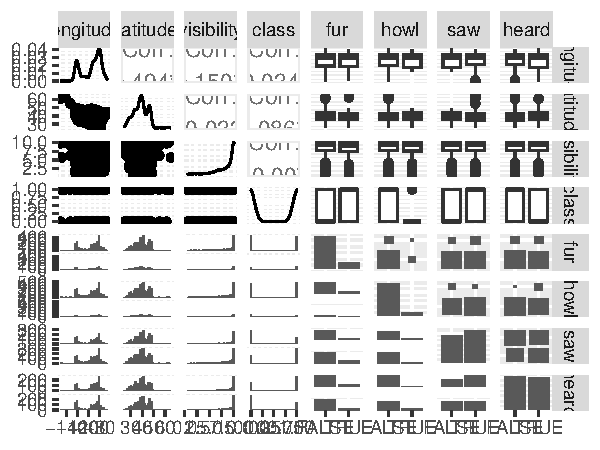
\includegraphics{Compulsory-1_files/figure-latex/unnamed-chunk-14-1} \end{center}

\begin{Shaded}
\begin{Highlighting}[]
\CommentTok{\# Splitting intro training and testing set}
\FunctionTok{set.seed}\NormalTok{(}\DecValTok{2023}\NormalTok{)}
\CommentTok{\# 70\% of the sample size for training set}
\NormalTok{training\_set\_size }\OtherTok{\textless{}{-}} \FunctionTok{floor}\NormalTok{(}\FloatTok{0.7} \SpecialCharTok{*} \FunctionTok{nrow}\NormalTok{(bigfoot))}
\NormalTok{train\_ind }\OtherTok{\textless{}{-}} \FunctionTok{sample}\NormalTok{(}\FunctionTok{seq\_len}\NormalTok{(}\FunctionTok{nrow}\NormalTok{(bigfoot)), }\AttributeTok{size =}\NormalTok{ training\_set\_size)}
\NormalTok{train }\OtherTok{\textless{}{-}}\NormalTok{ bigfoot[train\_ind, ]}
\NormalTok{test }\OtherTok{\textless{}{-}}\NormalTok{ bigfoot[}\SpecialCharTok{{-}}\NormalTok{train\_ind, ]}
\end{Highlighting}
\end{Shaded}

\hypertarget{a-2}{%
\subsubsection{a)}\label{a-2}}

In this subproblem we will consider a logistic regression model for our
task.

\hypertarget{i-3}{%
\paragraph{i)}\label{i-3}}

Below we fit a LRM and perform classification on our model using a 0.5
cutoff.

\begin{Shaded}
\begin{Highlighting}[]
\NormalTok{log\_reg\_mod }\OtherTok{\textless{}{-}} \FunctionTok{glm}\NormalTok{(class }\SpecialCharTok{\textasciitilde{}}\NormalTok{ ., }\AttributeTok{family =} \StringTok{"binomial"}\NormalTok{, }\AttributeTok{data =}\NormalTok{ train)}
\FunctionTok{summary}\NormalTok{(log\_reg\_mod)}
\end{Highlighting}
\end{Shaded}

\begin{verbatim}
## 
## Call:
## glm(formula = class ~ ., family = "binomial", data = train)
## 
## Deviance Residuals: 
##     Min       1Q   Median       3Q      Max  
## -2.0710  -1.0149  -0.4291   1.0007   2.1469  
## 
## Coefficients:
##              Estimate Std. Error z value Pr(>|z|)    
## (Intercept)  0.989051   0.422048   2.343 0.019106 *  
## longitude   -0.003112   0.003460  -0.900 0.368374    
## latitude    -0.036988   0.009849  -3.756 0.000173 ***
## visibility  -0.005681   0.023686  -0.240 0.810449    
## furTRUE      0.575172   0.136328   4.219 2.45e-05 ***
## howlTRUE    -0.792152   0.189803  -4.174 3.00e-05 ***
## sawTRUE      1.291894   0.097630  13.233  < 2e-16 ***
## heardTRUE   -1.075540   0.099634 -10.795  < 2e-16 ***
## ---
## Signif. codes:  0 '***' 0.001 '**' 0.01 '*' 0.05 '.' 0.1 ' ' 1
## 
## (Dispersion parameter for binomial family taken to be 1)
## 
##     Null deviance: 2948.6  on 2126  degrees of freedom
## Residual deviance: 2509.9  on 2119  degrees of freedom
## AIC: 2525.9
## 
## Number of Fisher Scoring iterations: 4
\end{verbatim}

\begin{Shaded}
\begin{Highlighting}[]
\NormalTok{pred\_prob }\OtherTok{\textless{}{-}} \FunctionTok{predict}\NormalTok{(log\_reg\_mod, }\AttributeTok{newdata =}\NormalTok{ test, }\AttributeTok{type =} \StringTok{"response"}\NormalTok{)}
\NormalTok{pred\_log }\OtherTok{\textless{}{-}} \FunctionTok{ifelse}\NormalTok{(pred\_prob }\SpecialCharTok{\textgreater{}=} \FloatTok{0.5}\NormalTok{, }\DecValTok{1}\NormalTok{, }\DecValTok{0}\NormalTok{)}
\NormalTok{obs }\OtherTok{\textless{}{-}} \FunctionTok{sum}\NormalTok{(pred\_log)}
\NormalTok{total\_obs }\OtherTok{\textless{}{-}} \FunctionTok{length}\NormalTok{(pred\_log)}
\end{Highlighting}
\end{Shaded}

We see that 441 are clear sightings out of our total sightings, which
are 912. \#\#\#\# ii) The short answer here is the coefficient
corresponding to the ``saw''-variable above, which is 1.292, i.e.~we
multiply by 1.292. Below we also have an approach for how to solve this
if we were instead provided with the coefficients from the
glmmet-function for this problem:

We start with our expression for odds \[
\frac{p}{1-p} = \frac{\frac{1}{1+e^{-U}}}{1-\frac{1}{1+e^{-U}}} = \frac{1}{1 + e^{-U} - 1} = e^U
\] Where \[
U = x^T \beta
\] \[
\frac{p}{1-p} = e^{x^T \beta} = e^{\beta_0 + x_1 \beta_1 + ... + x_n \beta_n}
\] \[ 
\frac{\text{odds}(Y_i = 1 | saw = TRUE)}{\text{odds}(Y_i = 1 | saw = FALSE)} = e^{\beta_{saw}} = 1.2919
\] So we need to multiply our odds by 1.2919 if our observation contains
the word ``saw'' compared to when it does not.

\hypertarget{b-2}{%
\subsubsection{b)}\label{b-2}}

In this subproblem we will consider a QDA model for our classification.

\hypertarget{i-4}{%
\paragraph{i)}\label{i-4}}

Below we fit a QDA model and perform classification, again with a 0.5
cutoff.

\begin{Shaded}
\begin{Highlighting}[]
\FunctionTok{library}\NormalTok{(MASS)}
\NormalTok{quadratic }\OtherTok{\textless{}{-}} \FunctionTok{qda}\NormalTok{(class }\SpecialCharTok{\textasciitilde{}}\NormalTok{ ., }\AttributeTok{data =}\NormalTok{ train)}
\NormalTok{prob\_quad }\OtherTok{\textless{}{-}} \FunctionTok{predict}\NormalTok{(quadratic, }\AttributeTok{newdata =}\NormalTok{ test)}\SpecialCharTok{$}\NormalTok{posterior  }\CommentTok{\#Posterior is a Nx2 matrix where each row is to be interpreted as the probability for that observation to be in the class A (first element) or class B (second element)}
\NormalTok{pred\_quad }\OtherTok{\textless{}{-}} \FunctionTok{predict}\NormalTok{(quadratic, }\AttributeTok{newdata =}\NormalTok{ test)}\SpecialCharTok{$}\NormalTok{class  }\CommentTok{\#Can just use the class variable, as the default is a cutoff of 0.5}
\NormalTok{obs2 }\OtherTok{\textless{}{-}} \FunctionTok{sum}\NormalTok{(}\FunctionTok{as.numeric}\NormalTok{(}\FunctionTok{as.character}\NormalTok{(pred\_quad)))}
\FunctionTok{summary}\NormalTok{(quadratic)}
\end{Highlighting}
\end{Shaded}

\begin{verbatim}
##         Length Class  Mode     
## prior    2     -none- numeric  
## counts   2     -none- numeric  
## means   14     -none- numeric  
## scaling 98     -none- numeric  
## ldet     2     -none- numeric  
## lev      2     -none- character
## N        1     -none- numeric  
## call     3     -none- call     
## terms    3     terms  call     
## xlevels  0     -none- list
\end{verbatim}

We now have 626 good observations out of 912.

\hypertarget{ii-3}{%
\paragraph{ii)}\label{ii-3}}

For the multiple choice we think point 1 and 4 are true, while 2 and 3
are false. TRUE, FALSE, FALSE, TRUE

\hypertarget{c-2}{%
\subsubsection{c)}\label{c-2}}

Here we will consider a KNN model in order to solve our problem.

\hypertarget{i-5}{%
\paragraph{i)}\label{i-5}}

Below we fit a KNN model with \(k=25\), using the knn function from the
class package, in order to again do classification.

\begin{Shaded}
\begin{Highlighting}[]
\FunctionTok{library}\NormalTok{(class)}
\NormalTok{knnMod }\OtherTok{\textless{}{-}} \FunctionTok{knn}\NormalTok{(}\AttributeTok{train =}\NormalTok{ train, }\AttributeTok{test =}\NormalTok{ test, }\AttributeTok{cl =}\NormalTok{ train}\SpecialCharTok{$}\NormalTok{class, }\AttributeTok{k =} \DecValTok{25}\NormalTok{, }\AttributeTok{prob =} \ConstantTok{TRUE}\NormalTok{)}
\CommentTok{\# prob=True gives us the class probabilities which we will need in the ROC{-}plot}

\CommentTok{\# Classification:}

\NormalTok{obs3 }\OtherTok{\textless{}{-}} \FunctionTok{sum}\NormalTok{(}\FunctionTok{as.numeric}\NormalTok{(}\FunctionTok{as.character}\NormalTok{(knnMod)))}

\CommentTok{\# Below we work with the probabilities so that we can use them in the ROC{-}plot}
\NormalTok{index }\OtherTok{\textless{}{-}} \FunctionTok{which}\NormalTok{(knnMod }\SpecialCharTok{==} \DecValTok{0}\NormalTok{)}
\NormalTok{knnMod.probs }\OtherTok{\textless{}{-}} \FunctionTok{attributes}\NormalTok{(knnMod)}\SpecialCharTok{$}\NormalTok{prob}
\NormalTok{knnMod.probs[index] }\OtherTok{=} \DecValTok{1} \SpecialCharTok{{-}}\NormalTok{ knnMod.probs[index]}
\end{Highlighting}
\end{Shaded}

In this model, 441 observations were classified as class A.

\hypertarget{ii-4}{%
\paragraph{ii)}\label{ii-4}}

We could find the optimal k from cross validating when we train our
data. This means that we split our training data into a training set and
a validation set. We now train our model with multiple different k's and
investigate their error with different subsets of the validation data.
We then pick the k-value based on error and simplicity.

\hypertarget{d-2}{%
\subsubsection{d)}\label{d-2}}

Now we want to compare the performance of our models.

\hypertarget{i-6}{%
\paragraph{i)}\label{i-6}}

In our situation, we would argue that we are interested in prediction,
to automate the classification of reports. For prediction, all our
models are relevant, while for inference, logistic regression would be
preferred since its hard to evaluate the effect of the predictors in KNN
and QDA. Since our goal is prediction, we do not exclude any of the
three models.

\hypertarget{ii-5}{%
\paragraph{ii)}\label{ii-5}}

Below we make confusion matrices for the predictions performed on the
test sets in a)-c) and present them

\begin{Shaded}
\begin{Highlighting}[]
\FunctionTok{library}\NormalTok{(caret)}
\FunctionTok{print}\NormalTok{(}\StringTok{"Logistic regression"}\NormalTok{)}
\end{Highlighting}
\end{Shaded}

\begin{verbatim}
## [1] "Logistic regression"
\end{verbatim}

\begin{Shaded}
\begin{Highlighting}[]
\NormalTok{conf\_log }\OtherTok{\textless{}{-}} \FunctionTok{table}\NormalTok{(pred\_log, test}\SpecialCharTok{$}\NormalTok{class, }\AttributeTok{dnn =} \FunctionTok{c}\NormalTok{(}\StringTok{"Prediction"}\NormalTok{, }\StringTok{"Reference"}\NormalTok{))}
\FunctionTok{print}\NormalTok{(conf\_log)}
\end{Highlighting}
\end{Shaded}

\begin{verbatim}
##           Reference
## Prediction   0   1
##          0 323 148
##          1 142 299
\end{verbatim}

\begin{Shaded}
\begin{Highlighting}[]
\FunctionTok{paste}\NormalTok{(}\StringTok{"sensitivity : "}\NormalTok{, }\FunctionTok{sensitivity}\NormalTok{(conf\_log))}
\end{Highlighting}
\end{Shaded}

\begin{verbatim}
## [1] "sensitivity :  0.694623655913978"
\end{verbatim}

\begin{Shaded}
\begin{Highlighting}[]
\FunctionTok{paste}\NormalTok{(}\StringTok{"specificity : "}\NormalTok{, }\FunctionTok{specificity}\NormalTok{(conf\_log))}
\end{Highlighting}
\end{Shaded}

\begin{verbatim}
## [1] "specificity :  0.668903803131991"
\end{verbatim}

\begin{Shaded}
\begin{Highlighting}[]
\FunctionTok{print}\NormalTok{(}\StringTok{"QAD"}\NormalTok{)}
\end{Highlighting}
\end{Shaded}

\begin{verbatim}
## [1] "QAD"
\end{verbatim}

\begin{Shaded}
\begin{Highlighting}[]
\NormalTok{conf\_qad }\OtherTok{\textless{}{-}} \FunctionTok{table}\NormalTok{(pred\_quad, test}\SpecialCharTok{$}\NormalTok{class, }\AttributeTok{dnn =} \FunctionTok{c}\NormalTok{(}\StringTok{"Prediction"}\NormalTok{, }\StringTok{"Reference"}\NormalTok{))}
\FunctionTok{print}\NormalTok{(conf\_qad)}
\end{Highlighting}
\end{Shaded}

\begin{verbatim}
##           Reference
## Prediction   0   1
##          0 228  58
##          1 237 389
\end{verbatim}

\begin{Shaded}
\begin{Highlighting}[]
\FunctionTok{paste}\NormalTok{(}\StringTok{"sensitivity : "}\NormalTok{, }\FunctionTok{sensitivity}\NormalTok{(conf\_qad))}
\end{Highlighting}
\end{Shaded}

\begin{verbatim}
## [1] "sensitivity :  0.490322580645161"
\end{verbatim}

\begin{Shaded}
\begin{Highlighting}[]
\FunctionTok{paste}\NormalTok{(}\StringTok{"specificity : "}\NormalTok{, }\FunctionTok{specificity}\NormalTok{(conf\_qad))}
\end{Highlighting}
\end{Shaded}

\begin{verbatim}
## [1] "specificity :  0.870246085011186"
\end{verbatim}

\begin{Shaded}
\begin{Highlighting}[]
\FunctionTok{print}\NormalTok{(}\StringTok{"KNN"}\NormalTok{)}
\end{Highlighting}
\end{Shaded}

\begin{verbatim}
## [1] "KNN"
\end{verbatim}

\begin{Shaded}
\begin{Highlighting}[]
\NormalTok{conf\_knn }\OtherTok{\textless{}{-}} \FunctionTok{table}\NormalTok{(knnMod, test}\SpecialCharTok{$}\NormalTok{class, }\AttributeTok{dnn =} \FunctionTok{c}\NormalTok{(}\StringTok{"Prediction"}\NormalTok{, }\StringTok{"Reference"}\NormalTok{))}
\FunctionTok{print}\NormalTok{(conf\_knn)}
\end{Highlighting}
\end{Shaded}

\begin{verbatim}
##           Reference
## Prediction   0   1
##          0 386  85
##          1  79 362
\end{verbatim}

\begin{Shaded}
\begin{Highlighting}[]
\FunctionTok{paste}\NormalTok{(}\StringTok{"sensitivity : "}\NormalTok{, }\FunctionTok{sensitivity}\NormalTok{(conf\_knn))}
\end{Highlighting}
\end{Shaded}

\begin{verbatim}
## [1] "sensitivity :  0.83010752688172"
\end{verbatim}

\begin{Shaded}
\begin{Highlighting}[]
\FunctionTok{paste}\NormalTok{(}\StringTok{"specificity : "}\NormalTok{, }\FunctionTok{specificity}\NormalTok{(conf\_knn))}
\end{Highlighting}
\end{Shaded}

\begin{verbatim}
## [1] "specificity :  0.809843400447427"
\end{verbatim}

Sensitivity is true positive, in this case the proportion of
B-classifications which are true. Specificity is then the proportion of
true A-classifications. Ideally, this is as large as possible.

\hypertarget{iii}{%
\paragraph{iii)}\label{iii}}

Below we plot the ROC curves and present the AUC for each of our models.

\begin{Shaded}
\begin{Highlighting}[]
\FunctionTok{library}\NormalTok{(pROC)}
\NormalTok{roc\_log }\OtherTok{\textless{}{-}} \FunctionTok{roc}\NormalTok{(}\AttributeTok{response =}\NormalTok{ test}\SpecialCharTok{$}\NormalTok{class, }\AttributeTok{predictor =}\NormalTok{ pred\_prob, }\AttributeTok{direction =} \StringTok{"\textless{}"}\NormalTok{)}

\NormalTok{roc\_quad }\OtherTok{\textless{}{-}} \FunctionTok{roc}\NormalTok{(}\AttributeTok{response =}\NormalTok{ test}\SpecialCharTok{$}\NormalTok{class, }\AttributeTok{predictor =}\NormalTok{ prob\_quad[, }\DecValTok{2}\NormalTok{], }\AttributeTok{direction =} \StringTok{"\textless{}"}\NormalTok{)}
\NormalTok{roc\_knn }\OtherTok{\textless{}{-}} \FunctionTok{roc}\NormalTok{(}\AttributeTok{response =}\NormalTok{ test}\SpecialCharTok{$}\NormalTok{class, }\AttributeTok{predictor =}\NormalTok{ knnMod.probs, }\AttributeTok{direction =} \StringTok{"\textless{}"}\NormalTok{)}

\NormalTok{g }\OtherTok{=} \FunctionTok{ggroc}\NormalTok{(}\FunctionTok{list}\NormalTok{(roc\_log, roc\_quad, roc\_knn))}
\NormalTok{g }\SpecialCharTok{+} \FunctionTok{scale\_colour\_discrete}\NormalTok{(}\AttributeTok{name =} \StringTok{"Method"}\NormalTok{, }\AttributeTok{labels =} \FunctionTok{c}\NormalTok{(}\StringTok{"Log"}\NormalTok{, }\StringTok{"QDA"}\NormalTok{, }\StringTok{"KNN"}\NormalTok{))}
\end{Highlighting}
\end{Shaded}

\begin{center}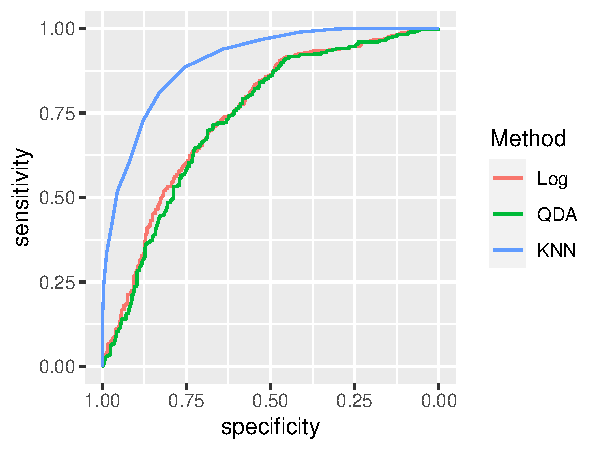
\includegraphics{Compulsory-1_files/figure-latex/unnamed-chunk-19-1} \end{center}

\begin{Shaded}
\begin{Highlighting}[]
\FunctionTok{paste}\NormalTok{(}\StringTok{"AUC {-} LOG: "}\NormalTok{, roc\_log}\SpecialCharTok{$}\NormalTok{auc)}
\end{Highlighting}
\end{Shaded}

\begin{verbatim}
## [1] "AUC - LOG:  0.745760265569748"
\end{verbatim}

\begin{Shaded}
\begin{Highlighting}[]
\FunctionTok{paste}\NormalTok{(}\StringTok{"AUC {-} QAD: "}\NormalTok{, roc\_quad}\SpecialCharTok{$}\NormalTok{auc)}
\end{Highlighting}
\end{Shaded}

\begin{verbatim}
## [1] "AUC - QAD:  0.73535878376753"
\end{verbatim}

\begin{Shaded}
\begin{Highlighting}[]
\FunctionTok{paste}\NormalTok{(}\StringTok{"AUC {-} KNN: "}\NormalTok{, roc\_knn}\SpecialCharTok{$}\NormalTok{auc)}
\end{Highlighting}
\end{Shaded}

\begin{verbatim}
## [1] "AUC - KNN:  0.901082485386447"
\end{verbatim}

\hypertarget{iv}{%
\paragraph{iv)}\label{iv}}

From the plot in iii) we see that the ROC for logistic regression and
quadratic discriminant analysis are rather similar, while the ROC for
our KNN model with \(k=25\) stands out. This is also confirmed by the
AUC-values, where KNN has the largest value. Since we want an AUC-value
as large as possible, we would here choose the KNN model.

\hypertarget{problem-4}{%
\section{Problem 4}\label{problem-4}}

\hypertarget{a-3}{%
\subsection{a)}\label{a-3}}

In this task we will consider the squared error for LOOCV:

\[
CV=\frac{1}{N}\sum_{i=1}^N(y_i-\hat{y}_{-i})^2
\] Now we can consider the second term, and aim to arrive at an
expression which involves our usual predictions, without LOOCV. We start
by using the first hint provided to us, namely that \[
\hat{y}_{-i}=\textbf{x}_i^\top \beta_{-i}
\] Where \(\beta_{-i}\) denotes the coefficient matrix for LOOCV and is
given by our usual formula for the coefficient matrix, i.e.: \[
\beta_{-i}=(\textbf{X}_{-i}^\top \textbf{X}_{-i})^{-1}\textbf{X}_{-i}^\top\textbf{Y}_{-i}
\]

Now, using the second hint for the inverse matrix, and the third hint
for the last matrix product to arrive at \[
\beta_{-i}=(\textbf{X}^\top\textbf{X}-\textbf{x}_i\textbf{x}_i^\top)^{-1}(\textbf{X}\textbf{Y}-\textbf{x}_iy_i)
\] If we now insert this in our expression for \(\hat{y}_{-i}\) and
combine with the Sherman-Morrison formula, which states that \[
(A+uv^\top)^{-1}=A^{-1}-\frac{A^{-1}u^\top A^{-1}}{1+v^\top A^{-1}u}
\] By combining with the fact that
\(h_i = \textbf{x}_i^\top\textbf{X}^\top\textbf{X}\textbf{x}_i\) \[
\begin{aligned}
\hat{y}_{-i} &= \textbf{x}_i^\top\left( (\textbf{X}^\top\textbf{X})^{-1} + \frac{\textbf{X}^\top\textbf{X}^{-1}\textbf{x}_i\textbf{x}_i^\top\textbf{X}^\top\textbf{X}}{1-\textbf{x}_i^\top\textbf{X}^\top\textbf{X}\textbf{x}_i} \right)(\textbf{X}^\top\textbf{Y}-\textbf{x}_iy_i) \\
&= \textbf{x}_i^\top(\textbf{X}^\top\textbf{X})^{-1}\textbf{X}^\top \textbf{Y} - \textbf{x}_i^\top(\textbf{X}^\top\textbf{X})^{-1}\textbf{x}_iy_i + \textbf{x}_i^\top\frac{\textbf{X}^\top\textbf{X}^{-1}\textbf{x}_i\textbf{x}_i^\top\textbf{X}^\top\textbf{X}}{1-h_i}\textbf{X}^\top\textbf{Y}-\textbf{x}_i^\top\frac{\textbf{X}^\top\textbf{X}^{-1}\textbf{x}_i\textbf{x}_i^\top\textbf{X}^\top\textbf{X}}{1-h_i}\textbf{x}_iy_i \\
&= \hat{y}_i - h_iy_i + \frac{h_i\hat{y}_i}{1-h_i} - \frac{h_i^2 y_i}{1-h_i} \\
& = \frac{\hat{y}_i-h_i\hat{y}_i - h_iy_i+h_i^2y_i+h_i\hat{y}_i-h_i^2 y_i}{1-h_i} \\
& = \frac{\hat{y}_i-h_iy_i}{1-h_i}
\end{aligned}
\] If we now finally plug this expression into our expression for the
MSE, we get that \[
\begin{aligned}
\text{CV}&=\frac{1}{N}\sum_{i=1}^N\left( y_i-\frac{\hat{y}_i-h_iy_i}{1-h_i}\right)^2 \\
&= \frac{1}{N}\sum_{i=1}^N\left( \frac{y_i-h_iy_i -\hat{y}_i+h_iy_i}{1-h_i}\right)^2 \\
&= \frac{1}{N}\sum_{i=1}^N\left( \frac{y_i -\hat{y}_i}{1-h_i}\right)^2 \quad \square
\end{aligned}
\]

\hypertarget{b-3}{%
\subsection{b)}\label{b-3}}

\hypertarget{i-7}{%
\paragraph{i)}\label{i-7}}

FALSE

\hypertarget{ii-6}{%
\paragraph{ii)}\label{ii-6}}

TRUE

\hypertarget{iii-1}{%
\paragraph{iii)}\label{iii-1}}

FALSE

\hypertarget{iv-1}{%
\paragraph{iv)}\label{iv-1}}

FALSE

\end{document}
